% Options for packages loaded elsewhere
\PassOptionsToPackage{unicode}{hyperref}
\PassOptionsToPackage{hyphens}{url}
%
\documentclass[
  11pt,
]{article}
\usepackage{amsmath,amssymb}
\usepackage{iftex}
\ifPDFTeX
  \usepackage[T1]{fontenc}
  \usepackage[utf8]{inputenc}
  \usepackage{textcomp} % provide euro and other symbols
\else % if luatex or xetex
  \usepackage{unicode-math} % this also loads fontspec
  \defaultfontfeatures{Scale=MatchLowercase}
  \defaultfontfeatures[\rmfamily]{Ligatures=TeX,Scale=1}
\fi
\usepackage{lmodern}
\ifPDFTeX\else
  % xetex/luatex font selection
\fi
% Use upquote if available, for straight quotes in verbatim environments
\IfFileExists{upquote.sty}{\usepackage{upquote}}{}
\IfFileExists{microtype.sty}{% use microtype if available
  \usepackage[]{microtype}
  \UseMicrotypeSet[protrusion]{basicmath} % disable protrusion for tt fonts
}{}
\makeatletter
\@ifundefined{KOMAClassName}{% if non-KOMA class
  \IfFileExists{parskip.sty}{%
    \usepackage{parskip}
  }{% else
    \setlength{\parindent}{0pt}
    \setlength{\parskip}{6pt plus 2pt minus 1pt}}
}{% if KOMA class
  \KOMAoptions{parskip=half}}
\makeatother
\usepackage{xcolor}
\usepackage[margin=1in]{geometry}
\usepackage{graphicx}
\makeatletter
\def\maxwidth{\ifdim\Gin@nat@width>\linewidth\linewidth\else\Gin@nat@width\fi}
\def\maxheight{\ifdim\Gin@nat@height>\textheight\textheight\else\Gin@nat@height\fi}
\makeatother
% Scale images if necessary, so that they will not overflow the page
% margins by default, and it is still possible to overwrite the defaults
% using explicit options in \includegraphics[width, height, ...]{}
\setkeys{Gin}{width=\maxwidth,height=\maxheight,keepaspectratio}
% Set default figure placement to htbp
\makeatletter
\def\fps@figure{htbp}
\makeatother
\setlength{\emergencystretch}{3em} % prevent overfull lines
\providecommand{\tightlist}{%
  \setlength{\itemsep}{0pt}\setlength{\parskip}{0pt}}
\setcounter{secnumdepth}{-\maxdimen} % remove section numbering
\usepackage{setspace}
\usepackage{float}
\usepackage{subfig}
\ifLuaTeX
  \usepackage{selnolig}  % disable illegal ligatures
\fi
\usepackage{bookmark}
\IfFileExists{xurl.sty}{\usepackage{xurl}}{} % add URL line breaks if available
\urlstyle{same}
\hypersetup{
  pdftitle={Differential Equation},
  pdfauthor={Roshan Rai},
  hidelinks,
  pdfcreator={LaTeX via pandoc}}

\title{Differential Equation}
\author{Roshan Rai}
\date{2024-07-18}

\begin{document}
\maketitle

\onehalfspacing

\textbf{This note contains parts that I learnt from the Differential
equation course of Rice university in edx.org. The code for rmarkdown
can be obtained
\href{https://raw.githubusercontent.com/Roshann-Rai/differential-equation/main/differential.Rmd}{\emph{https://raw.githubusercontent.com/Roshann-Rai/differential-equation/main/differential.Rmd}}}

\section{1. Differential Equation}\label{differential-equation}

A differential equation of simple form \(\frac{dy}{dt} + P(t)y = f(t)\)
explains how the change in one variable (independent variable) affects
the other dependent variable. It shows the direction of movement as well
as the magnitude of the movement of dependent variable with respect the
indpendent variable. It can be (i) ordinary differential equation that
has 1 independent variable, (ii) partial differential equation that has
at least 2 independent variables.

\subsection{1.1 Solution of differential
equation}\label{solution-of-differential-equation}

\textbf{a. General Solution} includes all the possible solutions that
typically includes arbitrary constant. For eg. \(y(t) = t^3 + c\) is a
general solution.\\
\textbf{b. Particular Solution} includes the solution without arbitrary
constant. Consider the intial condition: \[y(t_0) = 0\] \[c = 0\] So,
\[y(t) = t^3\] \clearpage

\begin{figure}

{\centering 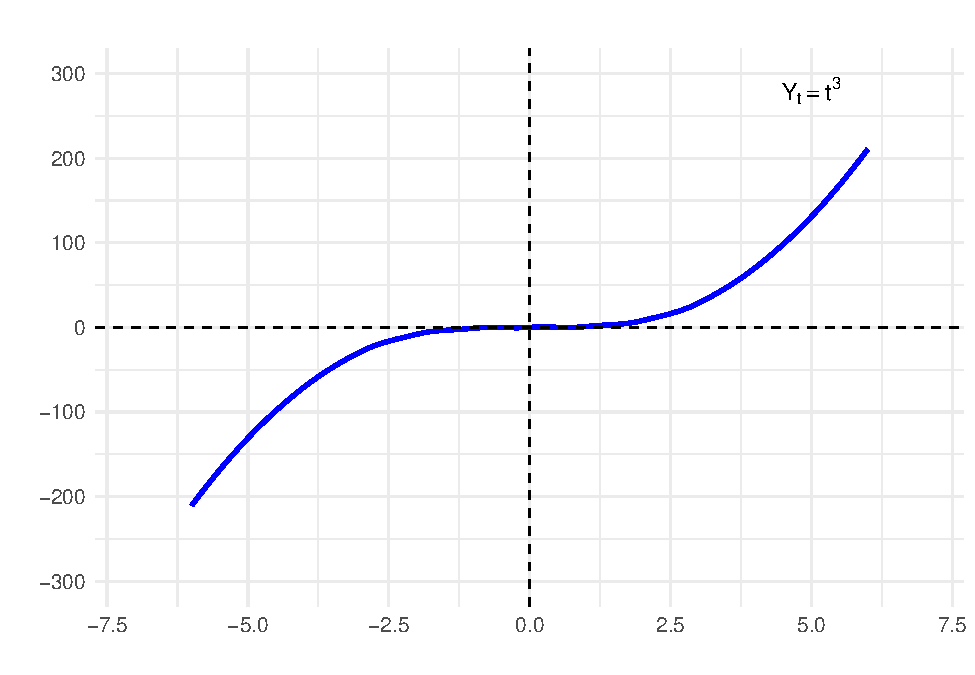
\includegraphics{differential_files/figure-latex/difference1-1} 

}

\caption{Plot of $y = t^3$}\label{fig:difference1}
\end{figure}

\subsection{1.2 Order of Differential
Equation}\label{order-of-differential-equation}

The order of the differential equation is the highest derivative of the
dependent variable that exists in the equation.
\[\frac{d^ny}{dt} = f(t, y^1, y^2,...., y^{n-1}, y^n)\] is the \(n-th\)
order differential equation.\\
First order differential equation is \[\frac{dy}{dt} = f(t, y)\]

\subsection{1.3 Directional Fields}\label{directional-fields}

Directional field also known as slope field is the graphical
representation of the solutions to the first order differential
equation. Consider the differential equation,
\[\frac{dy}{dt} = (y-2)(y+1)(1-y)^2\] To determine the directional
field, we equate the above equation equals to 0,
\[(y-2)(y+1)(1-y)^2 = 0\] So, \(y = 2, \pm1\). The graph is divided into
four regions i.e.~\(y <-1\), \(-1 < y < 1\), \(1 < y < 2\) and
\(y > 2\).\\
For, \(y < -1, \frac{dy}{dt} = 36\) when \(y = -2\),\\
For, \(-1 < y < 1, \frac{dy}{dt} = -1.05\) when \(y = -0.9\)\\
For, \(1 < y < 2, \frac{dy}{dt} = -0.0189\) when \(y = 1.1\)\\
For, \(y > 2, \frac{dy}{dt} = 0.3751\) when \(y = 2.1\)\\

\begin{figure}
\centering
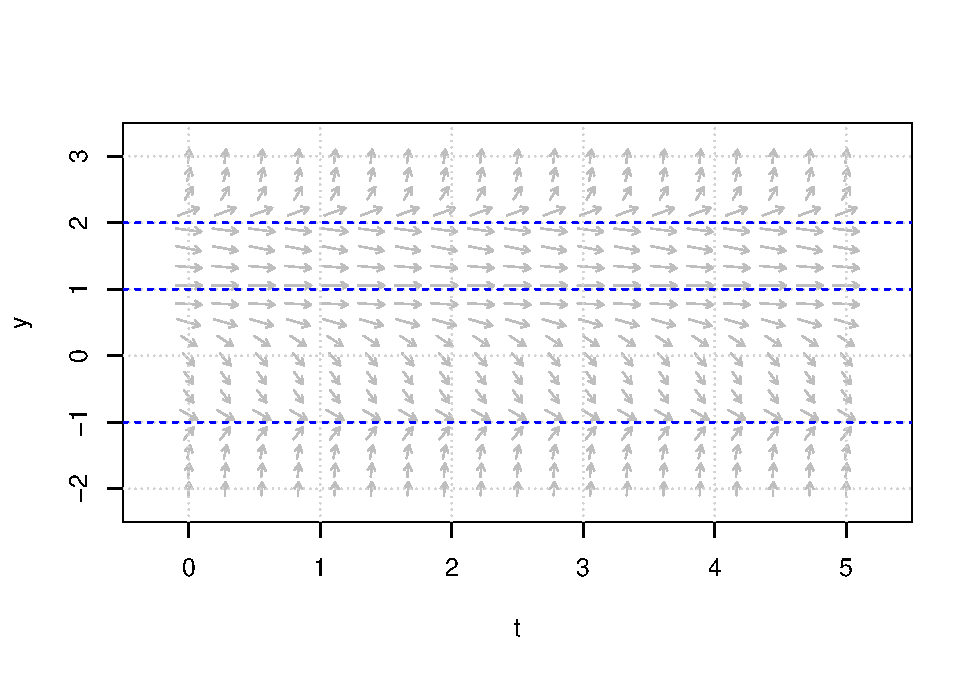
\includegraphics{differential_files/figure-latex/difference2-1.pdf}
\caption{Directional field of \(\frac{dy}{dt}=(y-2)(y+1)(1-y)^2\)}
\end{figure}

\subsection{1.4 Concavity}\label{concavity}

The graph of \(f(x)\) is concave up if \(f'(x)\) is increasing
i.e.~\(f'>0\) and concave down if \(f'(x)\) is decreasing
i.e.~\(f'(x)<0\).

\clearpage

\begin{figure}
\subfloat[Convex function (Concave upward)\label{fig:difference3-1}]{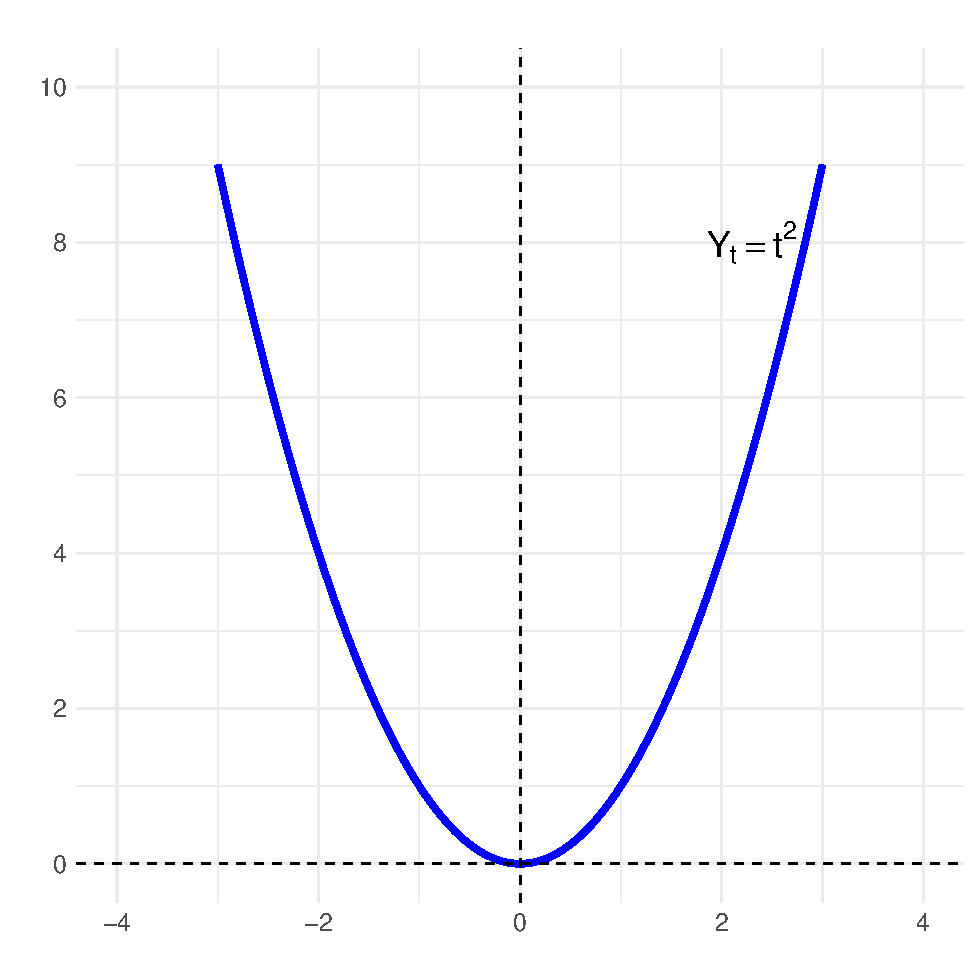
\includegraphics[width=.49\linewidth]{differential_files/figure-latex/difference3-1} }\subfloat[Concave function (Concave downward)\label{fig:difference3-2}]{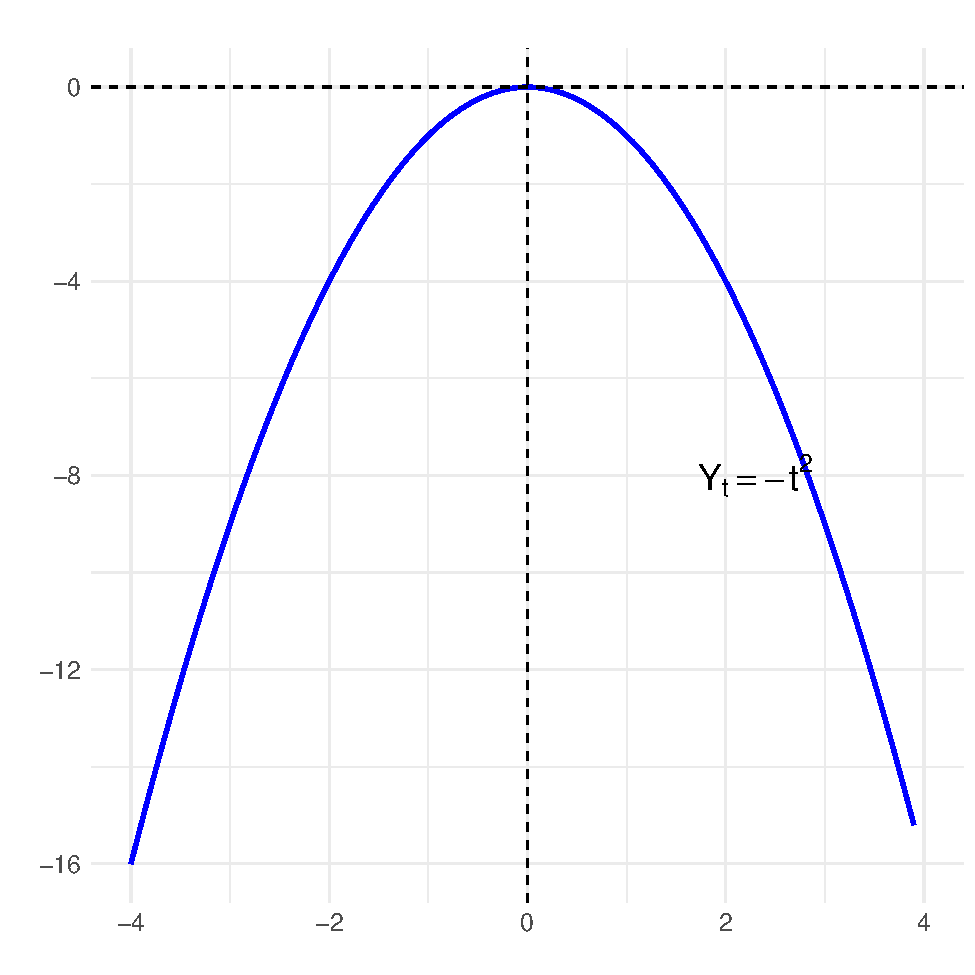
\includegraphics[width=.49\linewidth]{differential_files/figure-latex/difference3-2} }\end{figure}

\subsection{1.5 Separable equations}\label{separable-equations}

Differential equation is separable if \(y'=f(t)g(y)\).\\

\textbf{Example:} \[\frac{dy}{dt} = 3t^2(1+y)\]

\[
\frac{1}{1+y}dy = 3t^2dt \tag{1}
\]

\[
\int\frac{1}{1+y}dy = \int3t^2dt
\]

\[
ln|{1+y}|=t^3 + c
\]

\[
e^{ln|1+y|}=e^{t^3+c}
\]

\[
|1+y|=e^{t^3}.e^c 
\]

\[
1+y = \pm e^ce^{t^3} \tag{2}
\]

where \(e^c>0\) in equation (1).

\[
y = Ke^{t^3}
\]

\[
y = -1 + Ke^{t^3}
\]

\[
y = -1 + Ce^{t^3} \tag{3}
\]

In equation (3),

a. If \(C = 0\), \(y=-1\) is equilibrium solution.

b. If \(C \neq 0\), it gives all other possible solutions.

\textbf{Example:}

\[
\frac{dy}{dt}=\frac{3t^2+1}{1+2y}
\]

and \(y(0) = 1\)

The equation is in the form \(y'=f(t)g(y)\). So the equation can be
separated.

Does the equation has equilibrium solution?

Set, \(g(y) = 0\), \(\Longrightarrow\) \(\frac{1}{1+2y} = 0\). So, no
equilibrium solution.

Now,

\[
\int(1+2y)dy=\int(3t^2+1)dt
\]

\[
y+y^2=t^3+t+c \tag{1}
\]

Put \(y(0) = 1\), then \(C = 2\). So,

\[
y+y^2=t^3+t+2
\]

\[
(y^2+y)-(t^3+t+2)=0 \tag{2}
\]

Equation (2) is in the form of \(ax^2+bx+c = 0\), where \(a = 1\),
\(b = 1\) and \(c = -(t^3+t+2)\).

\[
y = \frac{-1\pm\sqrt{1+4(t^3+t+2)}}{2}
\]

\begin{figure}
\centering
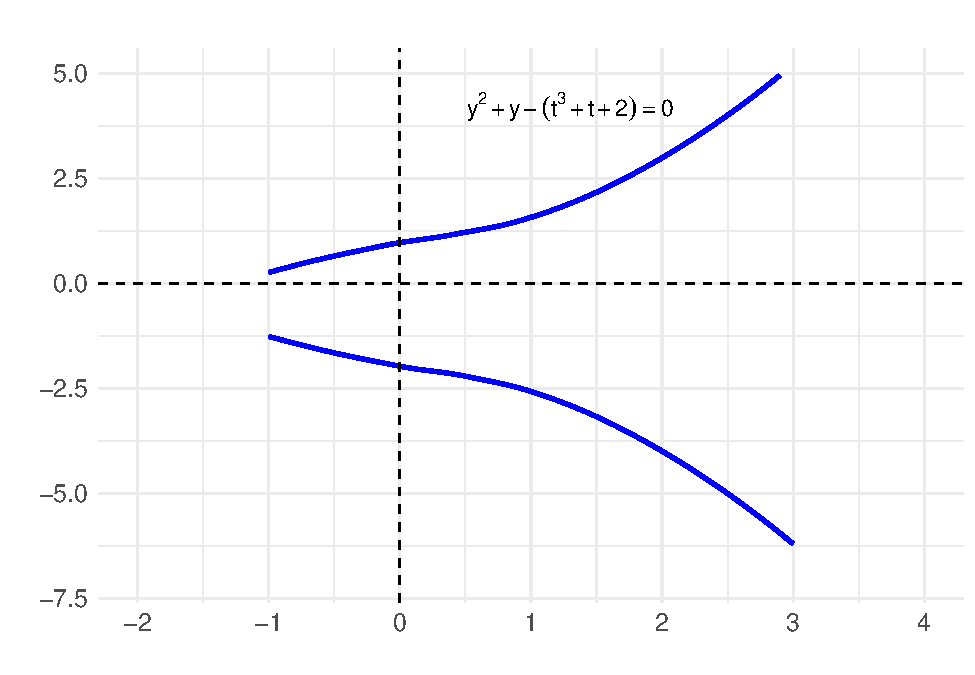
\includegraphics{differential_files/figure-latex/difference4-1.pdf}
\caption{Plot of \(y^2+y-(t^3+t+2)=0\)}
\end{figure}

\subsection{1.6 Picard's Theorem}\label{picards-theorem}

For \(y' = f(t,y)\) with \(y(t_0)=y_0\) to have solution:

\begin{itemize}
\tightlist
\item
  Condition I: f(t,y) should be continuous function\footnote{A function
    \(f(x)\) is continous at \(x=a\) if a. \(f(a)\) is defined, b.
    \(\lim_{x \to a} f(x)\) exists and c.~\(\lim_{x \to a} f(x) = f(a)\)}
  in a neighborhood of \(t_0,y_0\).
\item
  Condition II: The solution is unique if \(\frac{\delta f}{\delta y}\)
  is also continuous in neighbourhood of this initial condition \(t_0\)
  and \(y_0\).\\
\end{itemize}

\subsection{1.7 Linearity vs
Non-linearity}\label{linearity-vs-non-linearity}

A linear differential equation is in the form \(y'+p(t)y=f(t)\) which is
a first order linear differential equation. Non-linear differential
equation can be \(y'y=cost\). Properties of linear equations are:

\begin{itemize}
\tightlist
\item
  \textbf{Superposition principle}: If \(y_1\) and \(y_2\) are
  homogeneous solutions, their linear combinations \(c_1y_1 + c_2y_3\)
  is also homogeneous.
\item
  \textbf{Non homogeneous principle}: General solution for
  non-homogeneous equation is \(y(t) = y_P + y_H\) where \(y_P\) is
  solution for non-homogeneous equation and \(y_H\) is solution for
  homogeneous equation.
\end{itemize}

\newpage

\section{2. First order Differential
Equation}\label{first-order-differential-equation}

\subsection{2.1 First order linear non-homogeneous Equation: Variation
of
Parameters}\label{first-order-linear-non-homogeneous-equation-variation-of-parameters}

Consider the following first order ODE: \[y'+p(t)y=f(t) \tag{1}\] For
equation (1), \[y_H=Ce^{-\int{p(t)dt}} \tag{2}\] \[y_p=vy_H \tag{3}\]
Can \(v\) be constant?\\
No, \(v\) can't be constant because if \(v\) is constant then \(y_p\) is
scalar multiplicative of \(y_H\). This won't solve the non-homogeneous
equation. \(v\) is non-constant function of \(t\) i.e.~\(v(t)\).

From equation (3), \[y_p'=(vy_H)' \longrightarrow v'y_H+vy_H'\] So, in
equation (1), \[v'y_H+vy_H'+p(t)vy_H=f(t)\]
\[v'y_H+v[y_H'+p(t)y_H]=f(t)\] where \(y'_H+p(t)y_H=0\) \[v'y_H=f(t)\]
\[v'=\frac{f(t)}{y_H}\] \[v=\int\frac{f(t)}{y_H}dt \tag{4}\] Equation
(4) gives \(v\).

\textbf{Example:} \[y'+\frac{1}{1+t}y=2\] \[y(0)=0, t\geq0\]
\[y_H=Ce^{-\int\frac{1}{1+t}dt}\] \[y_H=Ce^{-ln|1+t|}\]
\[y_H=Ce^{ln|1+t|^{-1}}\] \[y_H=C|1+t|^{-1}\]
\[y_H=\frac{C}{1+t} \tag{1}\] Here we only take +ve sign because
\(t\geq0\). \[y_P=vy_H\] \[v'=\frac{f}{y_H}\]
\[v'=\frac{f}{\frac{1}{1+t}}\] \[v'=2(1+t)\] where \(f=2\)
\[v=\int{2(1+t)}dt\] \[v=2t+t^2+c \tag{2}\] Now, \[y_P=(2t+t^2+c)y_H\]
\[y_P=\frac{(t^2+2t+c)}{1+t} \tag{3}\] Here, we don't need to write
\(c\) because we will get the constant from \(y_H\). General Solution is
\[y=y_P+y_H\] \[y=\frac{2t+t^2}{t+1}+\frac{C}{t+1} \tag{4}\] We know,
\(y(0)=0\) so, \[0=\frac{2*0+0^2}{0+1}+\frac{c}{0+1}\] \[c=0\] Hence,
\[y=\frac{2t+t^2}{t+1} \tag{5}\] Eqn (5) is case when \(t\neq-1\).
\newpage

\subsection{2.2 First order linear non-homogeneous equation: Integrating
Factors}\label{first-order-linear-non-homogeneous-equation-integrating-factors}

Consider the following \[y'+p(t)y=f(t) \tag{1}\] Multiply equation (1)
by \(\mu\), \[\mu y'+p(t)y\mu=f(t)\mu\] Assume, \(\mu p(t) = \mu'\)\\
Now, \[\mu y'+\mu' y=\mu f(t)\] \[(\mu y)'=\mu f(t)\]
\[\int{(\mu y)'dt}=\int{\mu f(t)dt}\] \[\mu y +c = \int{\mu f(t)dt}\]
\[y = \frac{\int{\mu f(t)dt}-c}{\mu} \tag{2}\] In eqn (2), since c is
unknown constant, we change the sign -ve to +ve.
\[y = \frac{\int{\mu f(t)dt}+c}{\mu} \tag{3}\] From our assumption,
\[\mu p(t)=\mu' \longrightarrow p(t)=\frac{\mu'}{\mu}\] On right hand
side, it is simply the natural log of \(\mu\). So, \[p(t)=(ln\mu)'\]
\[\int{p(t)dt}=\int{(ln\mu)' dt}\] \[\int{p(t)dt+k}=\ln\mu\]
\[\mu = e^{\int{p(t)dt}+k}\] \[\mu = e^ke^{\int{p(t)dt}}\]
\[\mu = Ke^{\int{p(t)dt}} \tag{4}\] where \(K=e^k\).\\
If we set the value of \(\mu\) in equation 3, we get y,
\[y = \frac{\int{Ke^{\int{p(t)dt}} f(t)dt}+c}{Ke^{\int{p(t)dt}}} \tag{5}\]

\textbf{Example} \[y' + \frac{1}{t+1}=2\] and \(y(0)=0, t \geq 0\)\\
We Know, \[\mu = e^{\int{p(t)dt}}\] \[\mu = e^{\int{\frac{1}{1+t}dt}}\]
\[\mu = e^{ln|1+t|}\] \[\mu = |1+t|\] \[\mu = t+1\] We only take
positive sign because \(t \geq 0\). \[(\mu y)' = \mu f(t)\]
\[(\mu y)' = 2\mu\] \[[(1+t)y]'=2(1+t)\]
\[\int{[(1+t)y]'dt}=\int{2(1+t)dt}\] \[(1+t)y=t^2+2t+c\]
\[y=\frac{t^2+2t}{t+1}+\frac{c}{t+1} \tag{1}\] Since, \(y(0)=0\) so,
\(c = 0\) in equation (1). Then, \[y(t)=\frac{t^2+2t}{t+1} \tag{2}\]
\newpage

\section{3. Second order Differential
Equation}\label{second-order-differential-equation}

General form of Second order differential equation is in the form

\[
ay''+by'+cy=f(t)
\]

\subsection{3.1 With constant
coefficient}\label{with-constant-coefficient}

To find \(y_H = Basis\) \({y_1, y_2}\) where \(y_1, y_2\) are two
linearly independent functions. \[y(t)=e^{\lambda t}\]
\[y'(t)=\lambda e^{\lambda t}\] \[y''(t)=\lambda^2 e^{\lambda t}\] Then,
\[a\lambda^2 e^{\lambda t} + b\lambda e^{\lambda t} + c e^{\lambda t} = 0\]
\[e^{\lambda t}(a\lambda^2 +b\lambda + c) = 0\] Since,
\(e^{\lambda t} \neq 0\) so, \[a\lambda^2 +b\lambda + c= 0\]
\[\lambda_{1,2} = \frac{-b\pm\sqrt{b^2-4ac}}{2a}\]

\begin{itemize}
\tightlist
\item
  \(b^2-4ac>0\) \(\Longrightarrow\) Real distinct roots
\item
  \(b^2-4ac=0\) \(\Longrightarrow\) Repeated roots
\item
  \(b^2-4ac<0\) \(\Longrightarrow\) Complex Roots
\end{itemize}

\end{document}
